\chapter{Implementation}

\tocdata{toc}{$\rightarrow$\textit{Jeremy Sztavinovszki}}
\section{General Architecture}
\textbf{Author: Jeremy Sztavinovszki}
\begin{figure}
	\centering

	\includegraphics[width=\textwidth]{img/RECT-Architecture}
	
	\caption{RECT's Architecture}
	\label{fig:rect-architecture}
\end{figure}

The general Architecture of RECT looks like \ref{fig:rect-architecture}. This is a high level overview of the RECT stack.
It shows, that multiple client programs using the libraries provided for RECT send data through gRPC to the \textit{RECT-Backend},
which then handles sending the data to peers. The \textit{RECT-Backend} may also receive data for a Client process, which it will then
send to the corresponding client program through gRPC.
The following sections will go into more detail about the different parts of the stack and how they were implemented. 

\begin{figure}
	\centering

	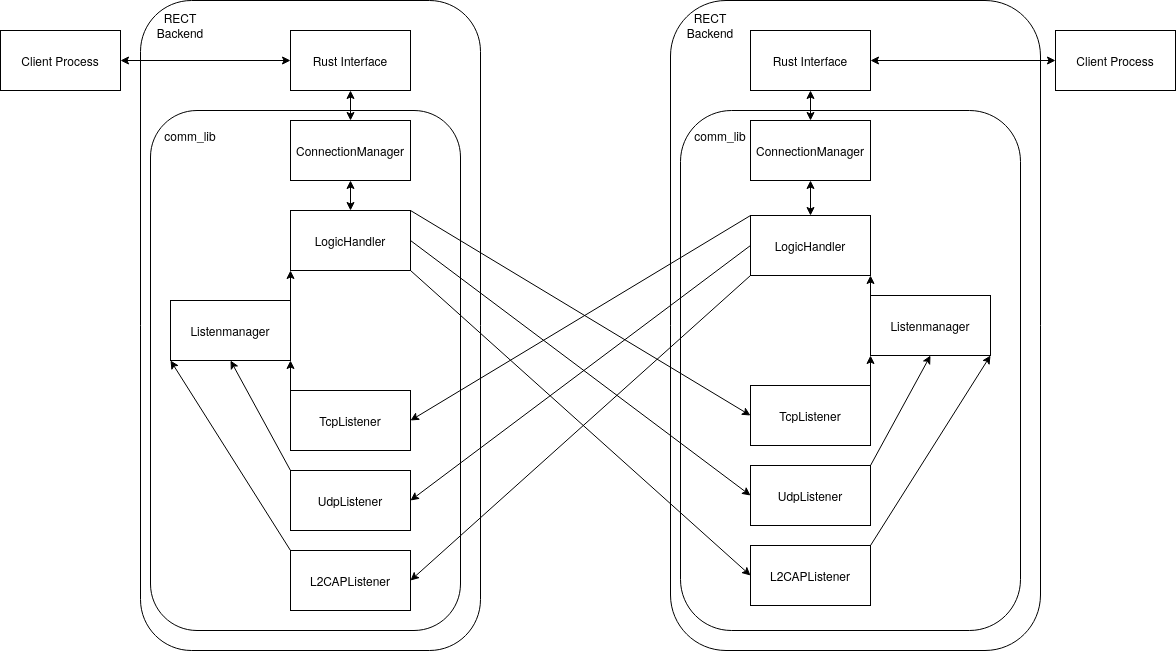
\includegraphics[width=\textwidth]{img/RECT-dataflow}

	\caption{The Flow of Data in RECT}
	\label{fig:rect-dataflow}

\end{figure}

\ref{fig:rect-dataflow} shows how data is sent through the different protocols in RECT.
In this diagram the \textit{RECT-Interface} handles the inter process communication with the client programs. 
The \textit{RECT-Interface} then interacts with components the comm\_lib, mainly the ConnectionManager, which is responsible for
handling the connections to the database and the LogicHandler. The LogicHandler is responsible for handling the logic for 
sending and receiving the different types of messages. It receives the messages from the ListenManager, which listens on the different
interfaces for incoming messages. The LogicHandler is also directly responsible for sending the messages through the different interfaces.
The following section covers these components in more detail.


\tocdata{toc}{$\rightarrow$\textit{Jeremy Sztavinovszki}}
\section{CommLib}
\textbf{Author: Jeremy Sztavinovszki} 
The Communication Library, or CommLib for short is the part of the RECT stack, that handles all of the communication between the hosts over traditional protocols, like TCP, UDP and BLE.
This requires it to be especially performant. For this reason a highly concurrent design was chosen, which uses the tokio library for asynchronous IO and the bluer library for Bluetooth communication. 
All of the communication between the components of the CommLib is done through tokio's channels, which means each component can be started and then run parallel to the other components.

\subsection{Setting up the Library} 
The first steps of setting up the library are more or less the same as in any other rust project. First the project is initialized with \verb+cargo new --lib <rust-name>+. This creates a
new folder with the name specified in \verb+<library-name>+ and generates some files like Cargo.toml and src/main.rs. After this step is done the needed libraries for RECT are added to the
project through \verb+cargo add <dependency-name> -F <dependency-name>/<feature-name>+ these dependencies are the pulled and built by cargo (Rust's build tool) upon the initial build of the
project. The first iteration of the project then had the following dependencies:

\begin{itemize}
	\item tokio
	\item bluer
	\item anyhow
\end{itemize}

All in all the commands used to generate the CommLib project and install all dependencies looked like this:
\newline
\begin{minipage}{\textwidth}
	\begin{lstlisting}[language=bash, caption=Setup Commands for CommLib]
		cargo new --lib CommLib && cd CommLib
		cargo add tokio bluer anyhow enum_dispatch -F tokio/full,bluer/full
		cargo build
	\end{lstlisting}
\end{minipage}

Any application using the CommLib needs to interact with this object in order to be able to use the communication methods provided by the library. 
To achieve this the CommLib provides the following functionality:

\begin{itemize}
	\item Setting a connection to a database, which is used to read the connections configured by the clients.
	\item Receiving simple messages, streams, requests and responses through any of the configured connections.
	\item Sending simple messages, streams, requests and responses through any of the configured connections.
	\item Initiating an update of the connections, which checks changes in the configuration found in the database and the connections, that are currently active in the ConnectionManager.
\end{itemize}

In the following sections the implementation of these functionalities will be covered in more detail.

\subsection{Datatypes for Handling Communication}
% enum_dispatch beschreiben
% verschiedene Typen beschreiben
In order to have a simple and easy to use interface for the CommLib, the library uses a set of different 
types to handle the different kinds of event, which can occur during communication. These types are
as follows:

\begin{itemize}
  \item SimpleMessage
  \item SimpleMessage acknowledgement
  \item Stream subscribe
  \item Stream unsubscribe
  \item Stream data
  \item Request
  \item Request acknowledgement
  \item Response
  \item Response acknowledgement
\end{itemize}

These types are implemented as structs in the CommLib which are part of an enum called Message. This enum uses the enum\_dispatch library
in order to be able to run a set of functions defined in a trait on each of the different structs. Each of the scructs embodies a different
use which will be explained in the following sections.

\subsubsection{SimpleMessage}
The simple message contains a message\_id, which is a 64 bit unsigned integer, a message, which is a vector, or array of bytes,
and a topic which is a String. This message is used to send a message which does not require a response. 
The message\_id is used to identify the message for acknowledgement and to ensure that there are different acknowledgement hashes
for two messages which contain the same data. The topic is used to identify the message on the receiving end.

\subsubsection{SimpleMessage acknowledgement}
The simple message acknowledgement is used to acknowledge the receipt of a simple message. It contains an acknowledgement hash, which is computed
from the message\_id and the data of the message. This hash is then used to verify, that the message was received and insure, that the data in the
message is correct.

\subsubsection{Stream subscribe}
The stream subscribe message is quite minimalistic, only containing a topic, which is a String. This message is used to subscribe to a topic
on the receiving end. Upon receiving this message the recipient will include the sender in the list of subscribers for a given topic. 

\subsubsection{Stream unsubscribe}
Stream unsubscribe is similar to stream subscribe, but is used to unsubscribe from a topic. So instead of adding the sender to the list of subscribers
the recipient will remove the sender from the list of subscribers for a given topic.

\subsubsection{Stream data}
The stream data message is used to send data to a subscriber. This message contains a topic, as well as a message, which is a vector of bytes.

\subsubsection{Request}
The request message is used to send a request to a recipient. It contains a request\_id, which is a 64 bit unsigned integer, a topic, and data, 
which is a vector of bytes. The request\_id is used to identify the request for acknowledgement and to ensure that there are different acknowledgements 
for two requests which contain the same data for the same topic. The topic is used to identify the request on the receiving end and relay it
to the correct recipient process.

\subsubsection{Request acknowledgement}
Similar to the simple message acknowledgement, the request acknowledgement is used to acknowledge the receipt of a request. It contains an acknowledgement
hash, which is computed from the request\_id, topic and the data of the request. This hash is then used to verify, that the request was received and insure, 
that the data in the request is correct. 

\subsubsection{Response}
The response message is used to send a response to a request. It contains a response\_id, which is a 64 bit unsigned integer, a topic, and data,
which is a vector of bytes. The response\_id is used to identify the response for acknowledgment and to relay the response to the correct requesting
process. The topic is used to identify the response on the receiving end.

\subsubsection{Response acknowledgement}
The response acknowledgement is used to acknowledge the receipt of a response. It is the exact same as the request acknowledgement, except for the 
name, which is changed in order to differentiate between the two.


\subsection{Logic for Handling Communication}
% wie werden die verschiedenen Typen verwendet um die Kommunikation zu handlen
% welche software Komponenten gibt es um diese Datentypen zu verwenden 
Datatypes alone however are not enough to implement the handling of the communication.
The logic needed to handle the communication is implemented in a couple of different software components on the CommLib.
These components are highly concurrent and use many of the features of the tokio library in order to allow the parallel handling of many different tasks.
The compoments are:

\begin{itemize}
  \item ConnectionManager. This is the component handling the database and relaying the commands received over gRPC to the other components of the CommLib.
  \item LogicHandler. This is the component handling the logic for the different types of messages. It is responsible for keeping track of subscribers to streams
  and for packing the messages into the correct format for binary serialization and sending them over the corresponding protocol. It receives all messages received on
  any of the available interfaces (TCP, UDP, L2CAP) through the ListenManager. It also handles the logic for 
  acknowledgements and any future optimizations concerning communication.
  \item ListenManager. This is the central component for receiving data over the different protocols. It is responsible for setting up listeneres on all interfaces and
  for relaying any data received to the LogicHandler in the form of Message structs.
  \item The Listeners. These are the components responsible for listening on their respective interfaces and sending the data to the ListenManager. 
\end{itemize}

The following sections will cover the implementation of these components in more detail.

\subsubsection{The Listeners}
The listeners are a fairly simple component. They are passed a Notify\footcite{rust-notify} to receive the notification when to stop and a sender for an unbounded channel\footcite{rust-unbounded-channel}, 
which is used to send the data received on the interface with the corresponding address the data was received from. 
The listener can then be started in a new tokio task and will run asynchronously until it receives the notification to stop.
Normally there are three listeners running at the same time, one for each of the protocols TCP, UDP and L2CAP.

\subsubsection{The ListenManager}
The ListenManager is a bit more complex than the listeners. It is a singleton and is responsible for setting up the listeners on the correct ports and with the correct addresses
(and service uuids in the case of L2CAP). It is also responsible for converting the received data from the listeners from binary into the corresponding Message structs and adding
information on what interface the data was received from. This is then sent to the LogicHandler through an unbounded channel.

\subsubsection{The LogicHandler}
The LogicHandler is yet another singleton. It contains a bit more data and logic than the before mentioned components, because of its central role in the CommLib.
It holds and populates a hashmap of published topics and subscribers to said topics, which are stored in a Vector of address strings and types of the interfaces the
subscribers are connected to. It provides a few public Senders and Receivers in order to be let other components interact with it. There are a few wrapper functions
for these Senders and Receivers, which are used in order to reduce the complexity of interaction with the LogicHandler and reduce duplicate code.

\subsubsection{The ConnectionManager}
The ConnectionManager is the last of the singleton components in the CommLib. It is responsible for interacting with the RECT database and for resolving the topics, or connection
names received through gRPC to the corresponding addresses and interfaces. It also relays data received through interfaces back to gRPC, as well as
calling the correct functions in the LogicHandler.

\subsection{Facing Problems with Concurrency}
Although the comm\_lib's structure is designed to be highly concurrent, there are problems in the implementation, which couldn't be resolved in time for the comm\_lib to be finished.
The main problem is concurrently handling the sending and receiving of messages, while also having to wait for the acknowledgements for previous messages. This means, that while 
the Listeners for the interfaces, the ConnectionManager and most of the LogicHandler have been implemented, complex tasks like acknowledgements and streams have not been implemented fully.

\tocdata{toc}{$\rightarrow$\textit{Christoph Fellner}}
\section{RECT Database}
\textbf{Author: Christoph Fellner}

\subsection{Database Structure}

The RECT Database is designed like \ref{fig:db-architecture}. This is a Entity Relationship Diagram (ERD) that shows the structure of the database. The database implements a
classic star schema, with the connections table as the center of the star. The connections table is linked to the client, method and address tables.

\begin{figure}
	\centering

	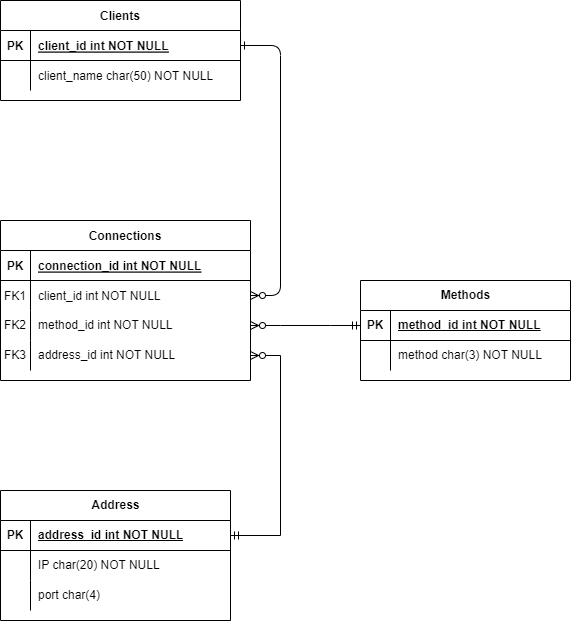
\includegraphics[width=\textwidth]{img/RECT-erd}

	\caption{Database Architecture of RECT.}
	\label{fig:db-architecture}
\end{figure}



The RECT database is structured according to the widely adopted star model, providing a robust framework for efficiently managing connection data. Comprising four distinct 
tables, namely connections, client, method, and address, this database architecture ensures comprehensive organization and accessibility of critical information.\newline

The connections table serves as a central hub, linking to the other three tables through their respective IDs and storing unique identifiers for each connection. 
Meanwhile, the client table houses data pertaining to the clients associated with specific connections, facilitating targeted access to connection information. In the 
method table, precisely three objects—BLE (Bluetooth Low Energy), TCP (Transmission Control Protocol), and UDP (User Datagram Protocol)—are stored, representing the 
available connection types within the RECT ecosystem. Additionally, the address table stores essential network information, including IP addresses and ports, with the 
provision for a null port value in instances where the connection method is BLE.\newline

By adopting this schema, the RECT database optimizes accessibility to connection data for clients by establishing seamless linkages between tables. Leveraging the Rusqlite
library, the backend components can efficiently query and retrieve pertinent information, enabling effective communication over the designated connections. Moreover, this 
database structure facilitates the extraction of various insights and metrics, empowering users to select and analyze data such as:

\begin{itemize}
  \item[] How many BLE, TCP or UDP connections are available?
  \item[] All connections of a specific client.
  \item[] All clients that have a specific connection.
  \item[] All connections that are available.
  \item[] How many connections are available in total?
  \item[] Are there more connections to the same client?
\end{itemize}

\subsection{Database usage}

The RECT Database serves as a vital resource accessible not only to the Rust Interface but also to the entirety of the backend infrastructure within the RECT stack. 
Acting as the backbone for data management, the Rust Interface undertakes the essential task of configuring the database, a process that includes the insertion of data 
sourced from the JSON file into its tables. This data encompasses a comprehensive inventory of available connections tailored specifically for the local RECT Client system.
Each connection within this dataset is meticulously characterized by a unique identifier, a designated communication method (be it BLE, TCP, or UDP), and a corresponding 
address composed of an IP address and port number.\newline

Upon completing the database setup and population with pertinent connection data, the backend components of the RECT stack rely on this repository to establish and manage 
communication channels. However, before the backend can effectively harness the capabilities of the database, the Rust Interface must first initialize the database setup 
and meticulously inject the JSON-derived information. Following this preparatory phase, the Interface seamlessly facilitates backend access to the database via the CommLib,
thereby ensuring a streamlined pathway for communication. Subsequently, armed with access to this centralized database, the backend components adeptly navigate and utilize
the provided connections to facilitate efficient communication processes tailored to the demands of the RECT ecosystem.

\tocdata{toc}{$\rightarrow$\textit{Christoph Fellner}}
\section{Rust Interface}
\textbf{Author: Christoph Fellner}

\begin{figure}
	\centering

	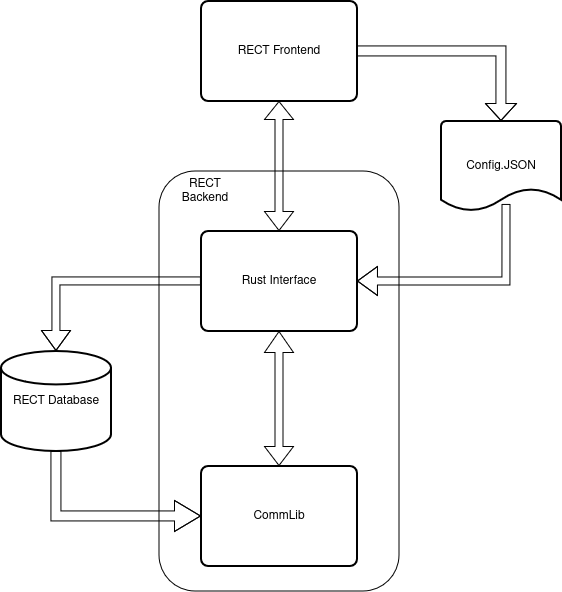
\includegraphics[width=\textwidth]{img/RustInterface}

	\caption{Structure of the Rust Interface.}
	\label{fig:rust-interface-architecture}
\end{figure}

One of the main sections of the RECT project is the Rust Interface. The Rust Interface is the part of the RECT stack that is responsible for the communication between 
the different parts of the stack. That means that the Rust Interface is responsible for the communication between the CommLib and the RECT Database. The RECT Database is 
part of the Rust Interface, it stores Data about all available RECT connections. The Rust Interface also communicates with the Python Service and the C++ Service. So 
basically the Rust Interface it responsible for the communication between the frontend and the backend of the RECT stack.\newline

In order to achieve this functionality the first step was to create a Rust module for gRPC communication. The gRPC communication is done with the help of the tonic library.
The tonic library is a gRPC library for Rust, which is based on the tokio library. The tokio library is a runtime for writing reliable asynchronous applications with Rust.
The gRPC module is responsible for the communication between the Rust Interface and the Python Service and the C++ Service. The gRPC module is also responsible for the 
communication between the Rust Interface and the CommLib.\newline 

The second step was to create a module for the RECT Database. The RECT Database is a in-memory SQLite database. The module uses the rusqlite library with the addition of
the tokio-rusqlite library. The tokio-rusqlite library is a asynchronous version of the rusqlite library. The Rust Interface implements the RECT Database, creates the 
necessary tables and provides the necessary functions to communicate with the database. The module is also responsible for the inserts of the available connections from a
JSON file into the database. The JSON file is created by the frontend and contains all available connections for the RECT stack.\newline

For the second step to work the Rust Interface also needs to be able to read the Config.JSON file in which the data for the connections is specified which in turn is stored 
in the rect database. The Config.JSON file is read by another module of the Rust Interface. The module uses the serde library to read JSON files. The serde library is a 
framework for serializing and deserializing Rust data structures efficiently and generically. The module defines suitable structures for the data strored in the JSON file 
and then reads the file and stores the data in the defined structures. The database module then takes this data and stores it in the RECT database.\newline

With these modules completed the Rust Interface is able to communicate with the CommLib, the Python Service and the C++ Service. In conclusion, the Rust Interface plays a 
crucial role within the RECT project, facilitating communication between various components of the stack. Through the implementation of modules for gRPC communication and 
the RECT Database, the Rust Interface ensures seamless interaction between the frontend and backend elements. Leveraging libraries such as tonic, tokio, rusqlite, and 
serde, the interface achieves reliable and efficient communication, handling tasks such as database management and data serialization effectively. Overall, the Rust 
Interface serves as a vital bridge, enabling smooth operation and integration within the RECT stack.

\section{C++ Implementation}
\textbf{Author: Maximilian Dragosits}
The C++ Implementation is one of the two outward facing components of the RECT stack. Alongside the Python Implementation 
it serves as a library in order for developers to be able to create robots, that are able to communicate with each other, much
easier then before. This is accomplished by abstracting most of the complexities of gRPC behind the \textit{Rectcpp} class. \\

The class only needs to be initialized with IP-Addresses for the different services that it offers and be given the IP of 
another of its kind and then it should be a simple act of using the predefined methods within the class in order to 
effortlessly communicate with other robots or devices running this or the Python frontend implementation.

\subsection{Rectcpp class}
The \textit{Rectcpp} class is the foundation of the C++ implementation, providing users with intuitive functions to control a diverse range of RECT services. 
These functions simplify the management of multiple gRPC services by condensing them into straightforward calls. 
For example, the listen method streamlines this process. With only one line of code, users can engage in listening activities while the underlying complexities are abstracted away. This encapsulation 
not only improves usability but also promotes efficient and robust utilization of RECT's capabilities, enabling developers to focus on their core objectives 
without being burdened by implementation details. An Example of this is the \textit{listen} function.

\begin{minipage}{\textwidth}
\begin{lstlisting}[language=c++]
  int Rectcpp::listen(std::string connectionName, std::string topic, std::string& returning);
\end{lstlisting}
\end{minipage}

The function requires users to provide the name of the connection to be monitored and specify the topic to which the incoming message must adhere. By supplying 
these parameters to the \textit{listen} function, users establish the criteria for message reception and filtration. When a message that meets the specified conditions 
arrives at the designated connection and aligns with the prescribed topic, it is retrieved. The function extracts the contents of the received message and 
returns them to the user as a string. This approach ensures a seamless and structured message handling process, allowing users to manage communication flows 
efficiently within the RECT framework.

There are two importent facets of this class aside from the simplified interaction with gRPC services. The hosting of its own services and the management of
connections to other services. The structure of \textit{Rectcpp} can be seen in this UML-Diagram:\\

\begin{figure}[H]
  \centering
	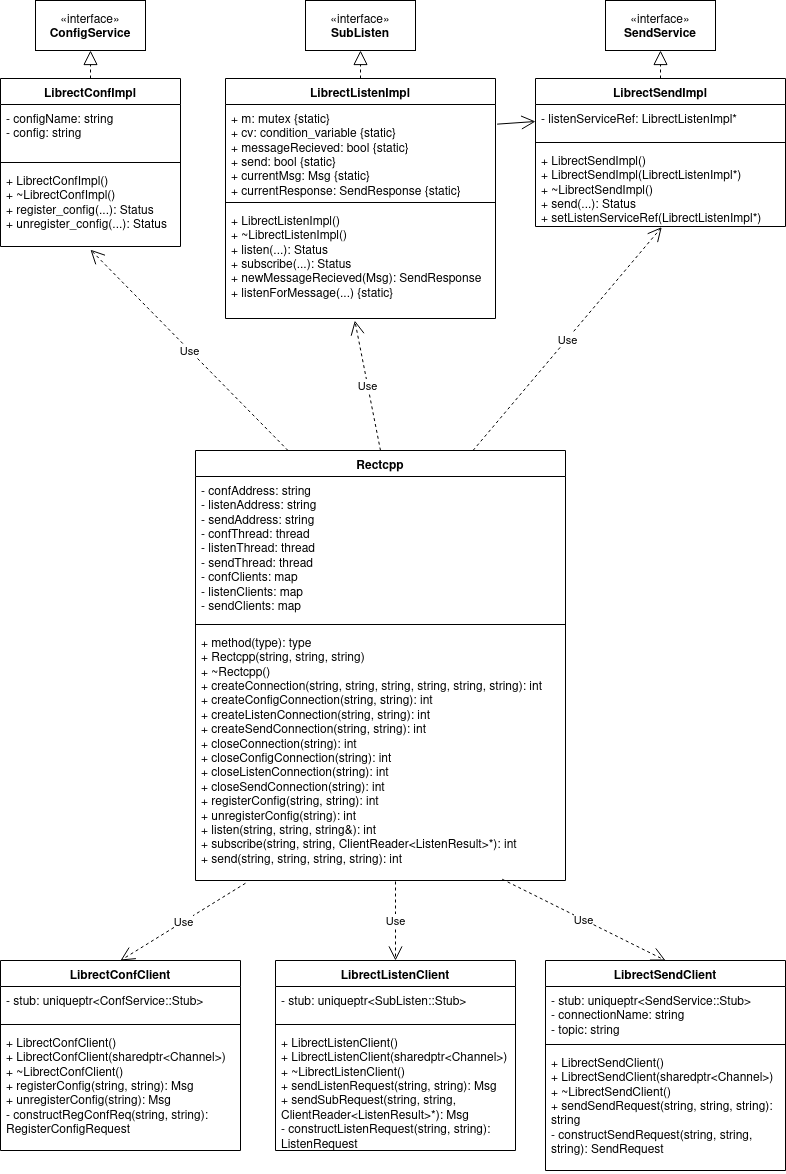
\includegraphics[width=\textwidth]{rectcpp_class_uml.png} 
	\caption{UML-Diagram of the \textit{Rectcpp} class}
	\label{fig:rectcppClassUML}
\end{figure}

While the users of the library will only directly interact with the methods of the main class, the various additional classes used in order to facilitate the
use of remote procedure calls are also displayed in the diagram. All the classes with the \textit{Impl} ending are the implementations of the interfaces automatically
generated by ProtoBuf and form the serves, that clients from other instances connect to. In contrast the \textit{Client} classes are for connecting to the servers
on other instances that host the relevant services.  

\subsubsection{Construction}
When invoking the constructor of the \textit{Rectcpp} class, users must provide the IP addresses and port numbers for the three distinct servers designated to launch the 
three different services. This crucial initialization step requires the network parameters to be provided in string format. The three services that are integral 
to this project are:  

\begin{itemize}
  \item{Config Service:} The Service used to send and recieve config data between two systems.
  \item{Listen Service:} The Service used to listen an subscribe to certain topics and then inform the listening clients when a message arrives.
  \item{Send Service:} The Service used to send messages with topics to other systems.
\end{itemize}

During the construction phase, instantiation of the services occurs, followed promptly by the commencement of a dedicated server for each. This initialization 
process is facilitated seamlessly through the utilization of the Serverbuilder module from the gRPC libraries, which streamlines the setup and configuration of 
servers. However, despite the robust capabilities of the gRPC Serverbuilder, challenges arose during the development of this library, primarily stemming from the absence 
of comprehensive documentation regarding the precise methodology for integrating the instantiated classes with the Serverbuilder module. This ambiguity led to 
several stumbling blocks and intricacies encountered along the path of development.

\subsubsection{Connections}
Connections within this class are managed using a C++ map structure, which allows for the binding of client instances to servers hosting the three services, 
all under user-assigned names. This approach significantly simplifies the usability of the class, replacing the need for cumbersome IP addresses and port 
numbers with easily discernible and memorable names. \\

The creation of connections is achieved through two distinct pathways: the general-purpose \textit{createConnection} function and its more specialized counterparts. 
The \textit{createConnection} function instantiates connections for all three services at once. In contrast, the more specific functions cater to individual service 
connections, depending on their designated name. For example, the \textit{createListenConnection} method requires only the name of the connection and the corresponding 
IP address. This establishes a connection solely with the Listen Service hosted at the provided address. This granular approach streamlines the process of 
establishing connections and enhances the modularity and flexibility of the Rectcpp class. Users can tailor their interactions with specific services according 
to their requirements.

\subsection{Definition of CMake file}
In order to compile and generate the gRPC services within this library CMake was used. The CMakeLists file of this project contains the standard CMake commands 
in order to make it into a C++ libary. Along side this are the lines responsible for ProtoBuf to generate the base classes for the implementation of gRPC. \\
First the proto files that will be turned into these base classes are registered using these lines: 

\begin{minipage}{\textwidth}
\begin{lstlisting}[caption=Excerpt from CMakeLists file of the C++ portion]
  file(GLOB RectVOneConf "${CMAKE_CURRENT_SOURCE_DIR}/proto/conf.proto")
  file(GLOB RectVOneListen "${CMAKE_CURRENT_SOURCE_DIR}/proto/listen.proto")
  file(GLOB RectVOneSend "${CMAKE_CURRENT_SOURCE_DIR}/proto/send.proto")
  file(GLOB RectVOneMessage "${CMAKE_CURRENT_SOURCE_DIR}/proto/message.proto")
  set(PROTO_CONF_FILES ${RectVOneConf})
  set(PROTO_LISTEN_FILES ${RectVOneListen})
  set(PROTO_SEND_FILES ${RectVOneSend})
  set(PROTO_MESSAGE_FILES ${RectVOneMessage})
\end{lstlisting}
\end{minipage}
The first three lines are for the files pertaining to the services and the last one is for the message type used by them in order to communicate. They are registered
using the \textit{file} command with the \textit{GLOB} keyword under a chosen name in order to refer back to them later in the CMake file. \\

After this each of the services is assigned a library using the \textit{add\_library} command and then the required dependencies for them to function are included using
\textit{target\_link\_libraries}. These are in this case \textit{libprotobuf}, \textit{grpc} and \textit{grpc++}.\\

Finally the \textit{protobuf\_generate} command is used to signify to ProtoBuf to generate the base classes when the project is built using CMake. 

\begin{minipage}{\textwidth}
\begin{lstlisting}[caption=Excerpt from CMakeLists file of the C++ portion]
  protobuf_generate(TARGET rect-conf-service LANGUAGE cpp)

  protobuf_generate(
      TARGET
        rect-conf-service
      LANGUAGE
        grpc 
      GENERATE_EXTENSIONS
        .grpc.pb.h
        .grpc.pb.cc
      PLUGIN 
        "protoc-gen-grpc=${grpc_cpp_plugin_location}"
  )
\end{lstlisting}
\end{minipage}
In this example the \textit{protobuf\_generate} is used twice. The first one sets the target files to be used during generation and the programming language 
for the classes to be created in. The second instance of the command informs it what type of service and the appropriate extensions for the generated files. 
The location of the gRPC generation plugin is also given.\\

This is then repeated for all of the services, that will be created. This is done in order to make it easier to implement gRPC within this library. 
The implementation of the classes generated by ProtoBuf is then accomplished by the manual creation of a class that extends the previously automatically 
created service class. This involves coding the functions that were originally defined within the proto files and then made into functions within the service classes.

\subsection{gRPC Serverbuilder}
During the development of the \textit{Rectcpp} class, a critical issue surfaced with the Serverbuilder\footcite{grpc_git_serverbuilder} provided by the gRPC library\footcite{grpc_git_documentation}. The problem stemmed from the method of 
passing the instance of the service to the builder, resulting in a compilation failure within the library. To ensure the smooth operation and continuous running of 
the servers, start functions were meticulously crafted for each of the three services. These functions employed threads containing lambda functions, responsible for 
initiating the servers and awaiting input from remote procedure calls. \\

Initially, all service classes were designated as private members of the main class and instantiated during its construction. Subsequently, these instances were 
passed to the functions responsible for spawning the server threads. However, the Serverbuilder\footcite{grpc_git_serverbuilder} employed in these functions could not accommodate this method of 
passing service objects.\\

The obscure and extensive error messages compounded the troubleshooting process, prolonging the resolution period. Consequently, numerous approaches were explored 
to access the pre-initialized objects within the start function, and notably within the lambda function executing the server thread. Techniques ranged from passing 
objects by reference to accessing class members from the function and copying them into new instances before passing them to the lambda functions. Regrettably, none 
of these strategies proved effective in resolving the issue. \\

After considerable effort, a breakthrough occurred when a simplified version of the \textit{Rectcpp} class was reconstructed. The pivotal realization was that 
constructing the service classes outside the lambda function was counterproductive. Instead, the solution lay in providing all necessary data for their initialization 
within the start functions, allowing them to be instantiated during the thread runtime. This adjustment finally circumvented the perplexing obstacle, enabling the 
starting of the servers.\\

\subsection{gRPC CreateChannel}
The other major issue that presented itself during development beside the problem with the Serverbuilder mentioned in the previous section is the throwing of a 
memory missmanegment error during runtime whenever the \textit{CreateChannel}\footcite{grpc_git_createchannel} function from the gRPC library\footcite{grpc_git_documentation} is called within the functions responsible for 
connecting a client to a server. \\

The specific line of code, that results in this error looks like this:
\begin{lstlisting}[language=C++]
  auto channel = CreateChannel(confAddress, InsecureChannelCredentials());
\end{lstlisting}
As can be seen a gRPC channel is returned by the function with a connection to the specified address. Here the IP-Address and Portnumber of the server to connect to
is contained within the variable \textit{confAddress} in the form of a string. The other argument signifies how the channel is to behave during use. During the execution
of the Rectcpp library one of two error messages appear in the console before the program shuts down. \\

\begin{minipage}{\textwidth}
\begin{lstlisting}[caption=One of the error messages of the Rectcpp class during execution]
  /home/maxi/rect/C++_Frontend/tests/main.cpp:51: FAILED:
    due to a fatal error condition:
    SIGSEGV - Segmentation violation signal
  ===============================================================================
  test cases: 1 | 1 failed
  assertions: 1 | 1 failed

  Segmentation fault
\end{lstlisting}

\begin{lstlisting}[caption=The other error message of the Rectcpp class during execution]
  terminate called after throwing an instance of 'std::bad_alloc'
  terminate called recursively
    what():  std::bad_alloc

  ~~~~~~~~~~~~~~~~~~~~~~~~~~~~~~~~~~~~~~~~~~~~~~~~~~~~~~~~~~~~~~~~~~~~~~~~~~~~~~~
  UnitTests is a Catch2 v3.4.0 host application.
  Aborted
\end{lstlisting}
\end{minipage}

The problem is that during the execution and use of the library a memory error called \textit{std::bad\_alloc} is invoked and the process is terminated. Because of 
the ambiguity of the error message the process of locating the source of the issue took a long time. After many failed attempts of resolving this issue it still
persists within the most recent version of the \textit{Rectcpp} library.\\

Unfortunatly a solution to this problem has proved to not be possible within the timeframe of the project. This has lead to the \textit{Rectcpp} class being 
largly not functional and not being able to connect to other instances of itself or instances of the Python library.

\subsection{Documentation}
Alongside the \textit{Rectcpp} library documentation has also been made for the functions of the library in order to make working with this tool easier in the future.
Unfortunatly the majority of this documentation in its current form will be useless due to the issues with the \textit{Rectcpp} class outlined in the previous paragraphs.
However it is still available in case someone in the future would like to continue developing this project.\\
This documentation was created with the help of \textit{Doxygen} and is accessible by looking wihtin the \textit{documentation} folder wihtin the project and opening
the \textit{Index.html} file in a browser. 

\tocdata{toc}{$\rightarrow$\textit{Timon Koch}}
\section{Python Implementation}
\textbf{Author: Timon Koch}

The Python Implementation and the C++ Implementation are the two primary components in the RECT stack that face outward. They serve as libraries that allow developers to create robots that can communicate seamlessly. The Rectpy class simplifies the usage of gRPC.

Initializing the class is as simple as providing IP addresses for its various services and specifying the IP of another instance. After initialization, developers can confidently use the pre-defined methods within the class to communicate seamlessly with other robots or devices running either this Python implementation or the C++ frontend.

\subsection{Rectpy class}
The Rectpy class forms the foundation of the Python implementation, providing users with powerful functions to efficiently control various RECT services. These functions streamline the management of multiple gRPC services by reducing them to simple calls. 

The send method requires only one line of code for users to send a message, abstracting away underlying complexities. This encapsulation improves usability and enables efficient and robust utilization of RECT's capabilities. Developers can focus on their core objectives without being burdened by implementation intricacies.

\begin{minipage}{\textwidth}
\begin{lstlisting}[language=python]
	def send(self, connectionName, msg, recipient, topic):
\end{lstlisting}
\end{minipage}

The function requires users to specify the connection to be monitored, the message itself, the recipient and the subject of the outgoing messages. By providing these parameters to the send function, users define the criteria for sending a message. This methodology ensures a seamless and structured message sending process, enabling efficient management of communication flows within the RECT framework.

It is also possible to receive messages from a given stream using the listen method. Like the send function, the listen method requires only a single line of code.

\begin{minipage}{\textwidth}
\begin{lstlisting}[language=python]
	def listen(self, connectionName, topic):
\end{lstlisting}
\end{minipage}

To receive a message, the Listen function requires the user to specify the connection to be monitored and the corresponding topic. By passing the necessary parameters to the function, the user defines the criteria for receiving messages. 

Two essential aspects of this class, besides the simplified interaction with gRPC services, are the hosting of own services and the management of connections to other services.

\subsubsection{Construction}
When initialising the Rectpy class constructor, users are required to provide the IP addresses and port numbers for the three different servers responsible for launching the three different services. This critical initialisation step requires the provision of network parameters in string format. The three services involved in this project are

\begin{itemize}
  \item{Config Service:} Facilitates the exchange of configuration data between two systems.
  \item{Listen Service:} Allows subscriptions to specific topics and notifies listening clients when messages arrive.
  \item{Send Service:} Allows messages with specified topics to be sent to other systems.
\end{itemize}

During the build phase, the services are instantiated, followed immediately by the launch of a dedicated server for each service. This initialisation process is seamlessly facilitated by the use of the Serverbuilder module from the gRPC libraries, which streamlines the setup and configuration of servers.

\subsubsection{Connection}

Connection creation is achieved in two different ways: the general purpose createConnection function and its more specialised counterparts. The createConnection function instantiates connections for all three services at once. The more specific functions, on the other hand, instantiate connections for individual services depending on the name given to them. For example, the createSendConnection method will only connect to the Send service hosted at the specified address. This granular approach streamlines the connection establishment process and increases the modularity and flexibility of the Rectpy class. Users can tailor their interactions with specific services according to their needs.

\subsection{Documentation}
In addition to the Rectpy library, extensive documentation has been created using Pydoc for its functions to facilitate future use of this tool. This documentation can be accessed by navigating to the documentation folder within the project directory and opening the associated file. 

\filbreak
